\section{Car-sharing services characterization} 
\label{sec:4_4_characterization}

In this section, we first present temporal characterization of the three services (section~\ref{sec:4_4_temporal_characterization}). Then, we describe the services spatial-temporal characteristics (section~\ref{sec:4_4_spatial-temporal}). Finally, we present users' behavior (section~\ref{sec:4_4_user-behavior}).

\subsection{Temporal characteristics}
\label{sec:4_4_temporal_characterization}


\begin{figure}
	\centering
	\subfloat[\centering Two-way Modo Weekdays]{{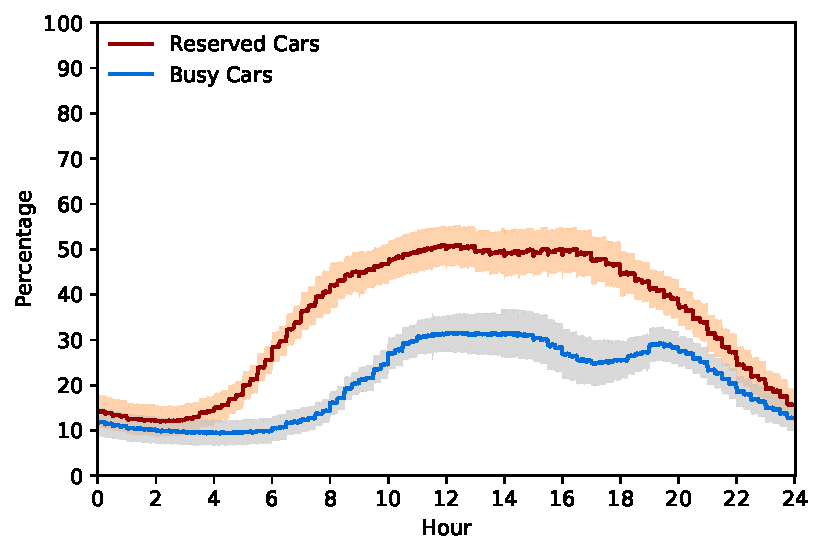
\includegraphics[width=0.46\columnwidth]{modo_inTravel/weekdays.pdf}} \label{fig:4_4_modo_wd}}%
	\qquad
	\subfloat[\centering Two-way Modo Weekends]{{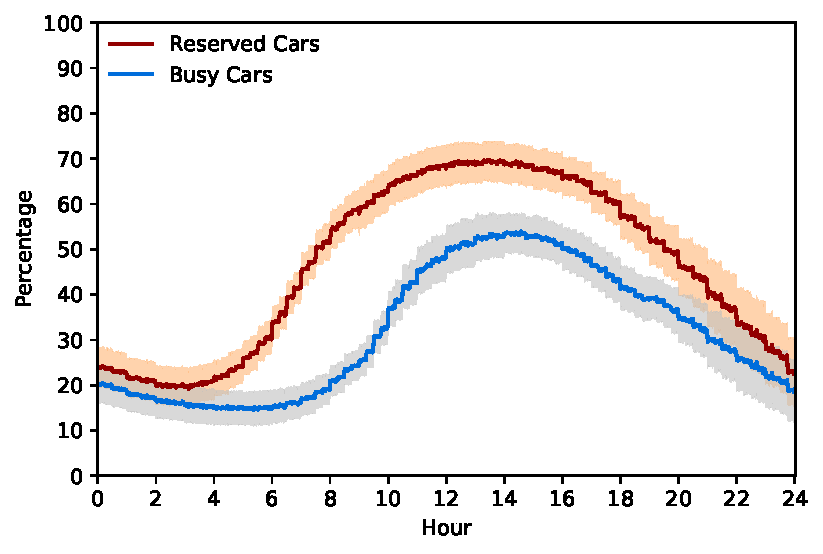
\includegraphics[width=0.46\columnwidth]{modo_inTravel/weekends.pdf}} \label{fig:4_4_modo_we}}%
	\caption{Modo Minute-by-minute mean value (plus/minus standard deviation) for  the  percentage of busy (blue curve) and reserved cars (red curve), for weekdays and weekends}
	\label{fig:4_4_modo_busy}%
\end{figure}


\begin{figure}
	\centering
	\subfloat[\centering One-way Evo Weekdays]{{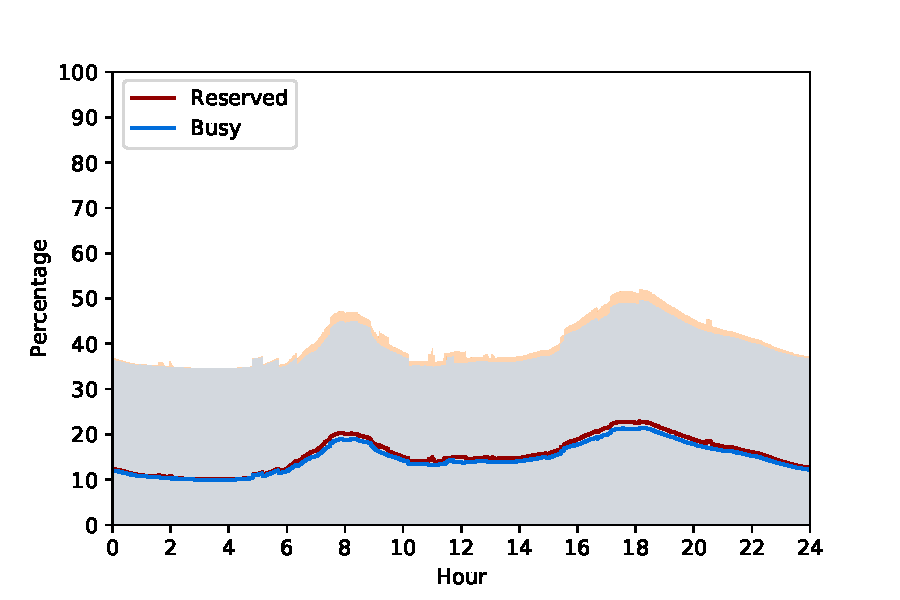
\includegraphics[width=0.46\columnwidth]{evo_inTravel/weekdayslim.pdf}} \label{fig:4_4_evo_wd}}%
	\qquad
	\subfloat[\centering One-way Evo Weekends]{{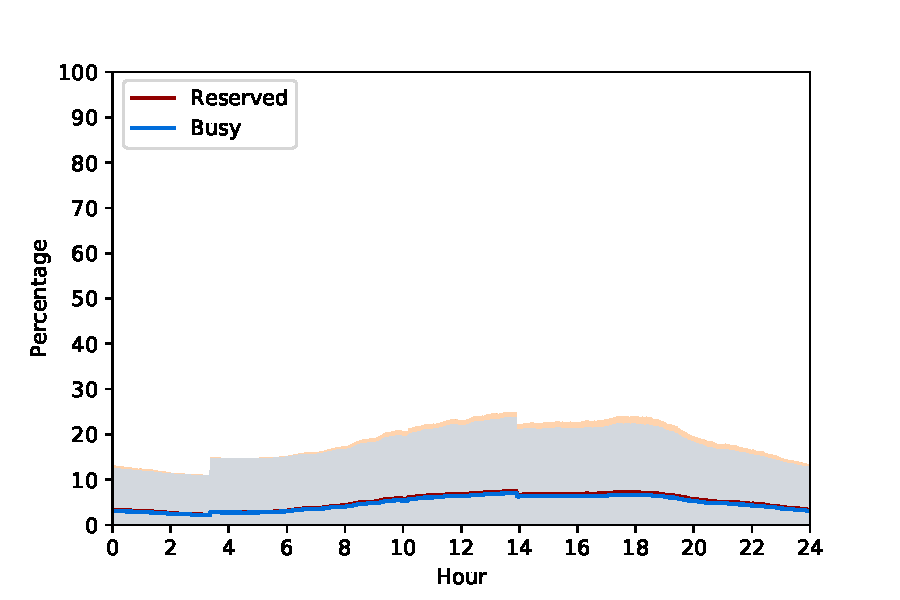
\includegraphics[width=0.46\columnwidth]{evo_inTravel/weekendslim.pdf}} \label{fig:4_4_evo_we}}%
	\caption{Evo Minute-by-minute mean value (plus/minus standard deviation) for  the  percentage of busy (blue curve) and reserved cars (red curve), for weekdays and weekends}
	\label{fig:4_4_evo_busy}%
\end{figure}

\begin{figure}
	\centering
	\subfloat[\centering Free floating car2Go Weekdays]{{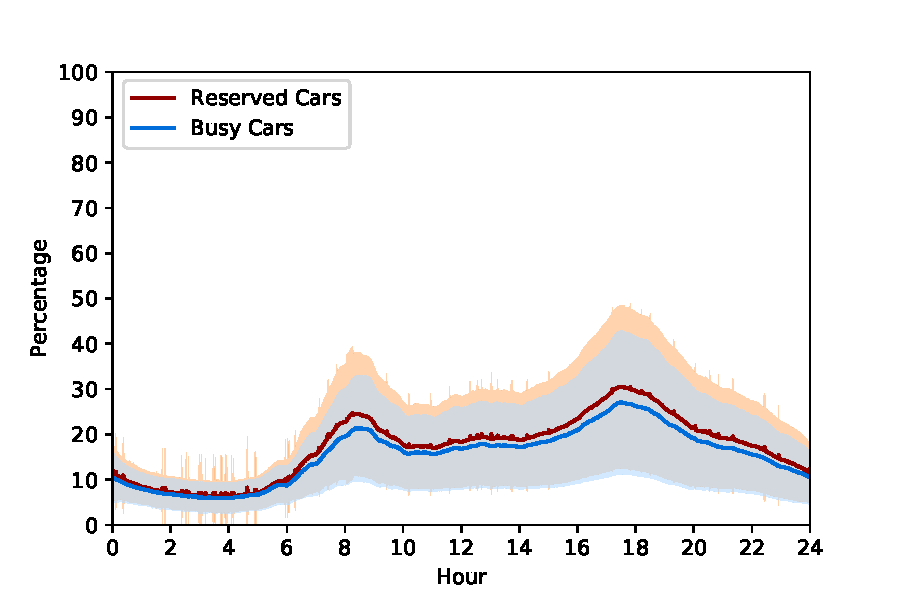
\includegraphics[width=0.46\columnwidth]{car2go_inTravel/weekdayslim.pdf}} \label{fig:4_4_c2g_wd}}%
	\qquad
	\subfloat[\centering Free floating car2Go Weekends]{{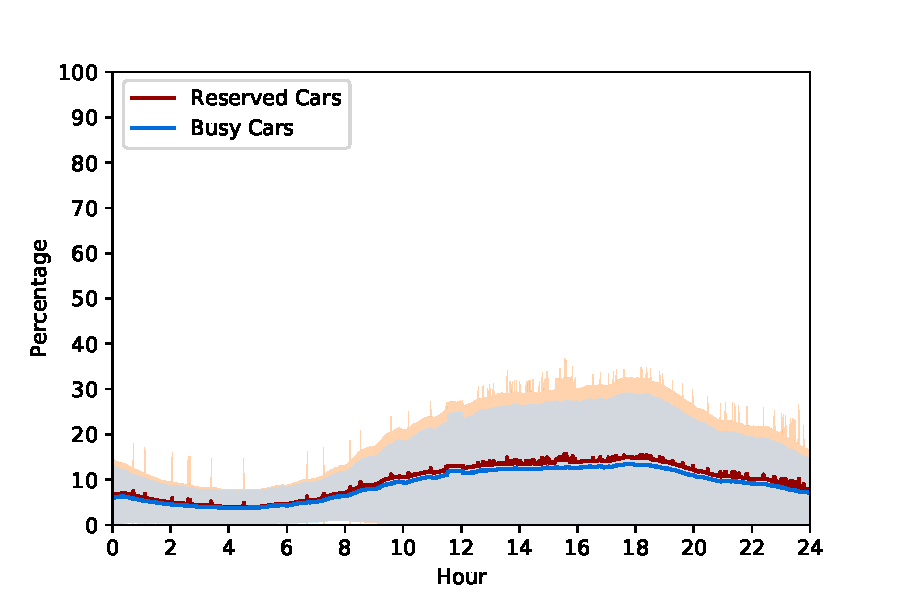
\includegraphics[width=0.46\columnwidth]{car2go_inTravel/weekendslim.pdf}} \label{fig:4_4_c2g_we}}%
	\caption{car2go Minute-by-minute mean value (plus/minus standard deviation) for  the  percentage of busy (blue curve) and reserved cars (red curve), for weekdays and weekends}
	\label{fig:4_4_c2g_busy}%
\end{figure}

%PRENSENTATION OF FIGURE
Figures~\ref{fig:4_4_modo_busy}, \ref{fig:4_4_evo_busy} and \ref{fig:4_4_c2g_busy} show the service daily demand pattern. In all plots, the blue and red solid lines refer to a minute-by-minute mean value over the studied period for the percentage of busy and reserved cars, respectively, for each service. The plots show also the standard deviation from the mean as the smoothed gray and orange background areas around the mean. On the left of each pair of figures (figures \ref{fig:4_4_modo_wd}, \ref{fig:4_4_evo_wd} and \ref{fig:4_4_c2g_wd}) is presented the demand pattern during working days, while on the (figures \ref{fig:4_4_modo_we}, \ref{fig:4_4_evo_we} and \ref{fig:4_4_c2g_we}) is shown the demand for weekends (Saturdays, Sundays, and festivities). 

%Overall, this figure highlights four main insights about the daily demand for the three services: (i) all of them present differences between weekdays and weekends; (ii) Modo has a distinct demand pattern when compared to the other two services; (iii) the number of cancellations is considerable in Modo and; (iv) the variation on demand, considering all analyzed period is small for Modo, but it is large for Evo and Car2go.

%DESCRIPTION OF INSIGHTS OF FIGURE
All three services present two peaks of demand during weekdays and only one during the weekends. During weekdays, for Evo and Car2Go, the one-way and free-floating services, the peaks of demand occur about 8~AM and 6~PM whereas for Modo, the two-way service, these peaks occur around 2~PM and 7~PM.
Moreover, note that for Evo and Car2Go, weekdays demand is higher than during weekends. On the other hand, for Modo, we observe just the opposite. 
Mostly, Modo users are regulars and present weekly/daily/hourly subscription. In this sense, they tend to reserve cars at the same hour, for regular periods, which explains Modo lower variation. For a given moment, we consider the relative difference between the reserved and busy cars as the cancellations of the system. Modo presents up to 60\% of cancellations, while the other two services present no more than 5\%. 
%For Modo, during weekdays, the cancellations often occur during all the day, including on the peak hours. During weekends, on the other hand, the number of cancellations is lower in the Modo peak of use. \lv{Not completely true from the plot}



\begin{figure}[htb]
\centering
    \begin{minipage}[b]{0.45\linewidth}
    \centering
     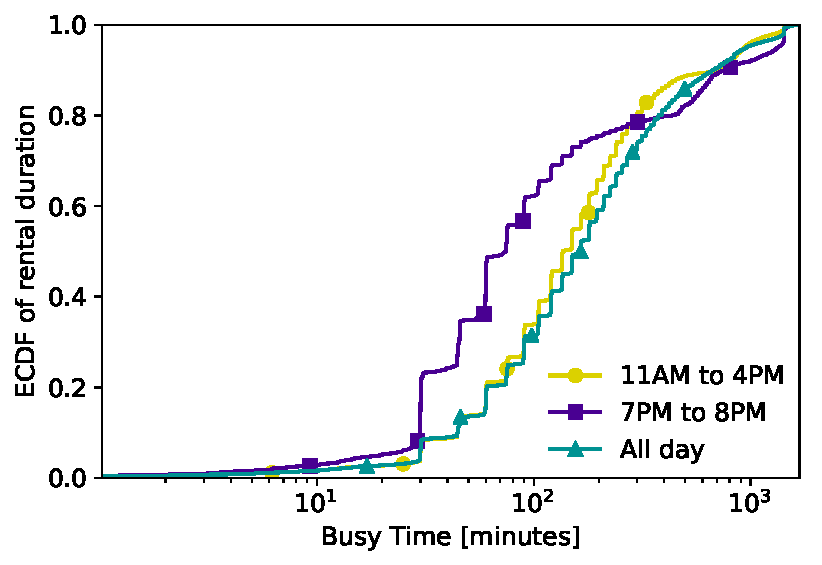
\includegraphics[width=59mm]{modo_cdfs/modo_tarde_noiteCDF_rebuttal.pdf}
     {\\(a) Two-way Modo}
    \end{minipage}
    \hspace{5mm}
    \begin{minipage}[b]{0.45\linewidth}
     \centering
     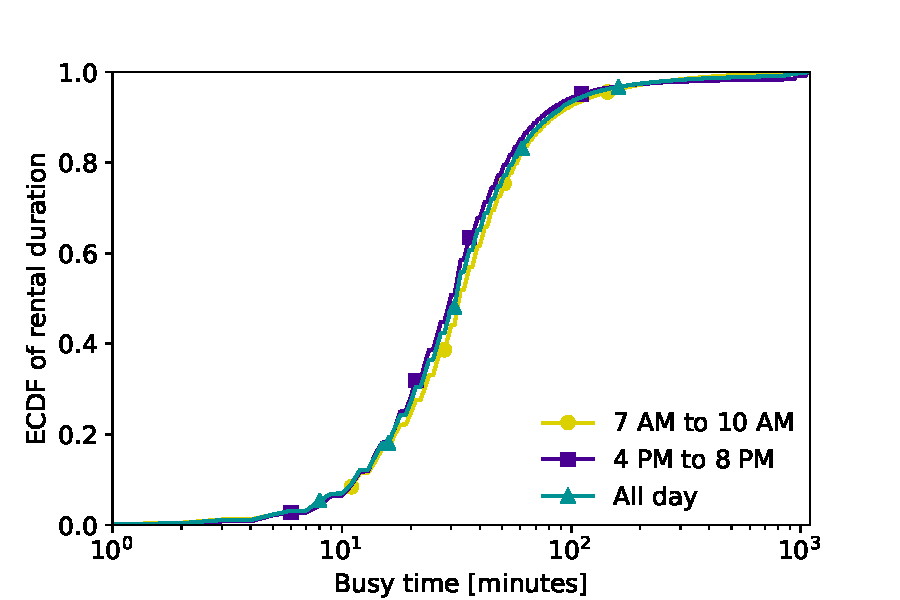
\includegraphics[width=65mm]{evo_cdfs/evo_tarde_noiteCDF_rebuttal.pdf}
     \vspace*{-3mm}
     {\\(b) One-way Evo}
    \end{minipage}
    %\hspace{1cm}
    %\hspace{5mm}
    \begin{minipage}[b]{0.45\linewidth}
    \vspace{5mm}
     \centering
     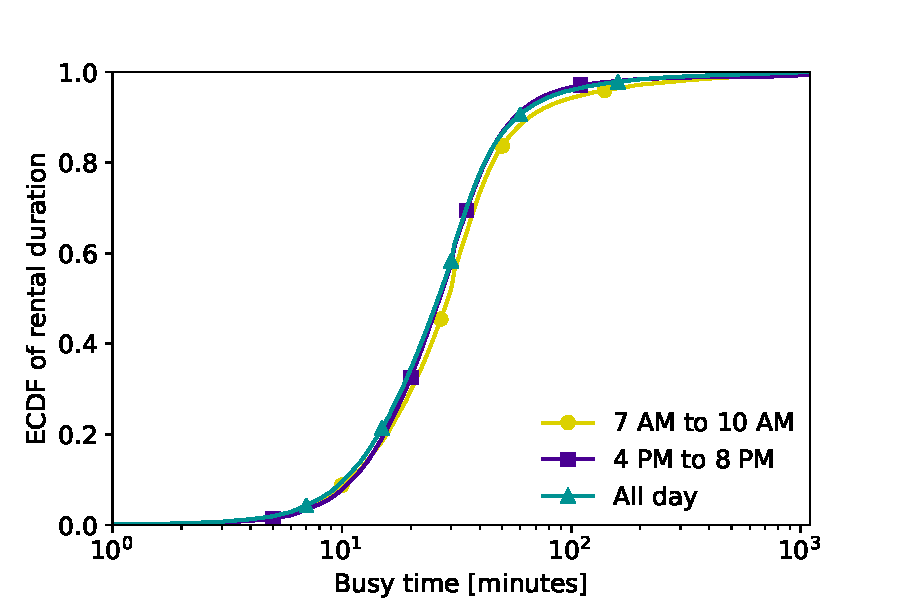
\includegraphics[width=65mm]{car2go_cdfs/c2g_tarde_noiteCDF_rebuttal.pdf}
     {\\(c) Free floating Car2Go}
    \end{minipage}
    \caption{Cumulative distribution function of vehicle busy time during a weekday.}
    \label{fig:4_4_cdfs_picos}
\end{figure}

%DESCRIPTION OF FIGURE
Figure~\ref{fig:4_4_cdfs_picos} presents the Empirical Cumulative Distribution Function (ECDF) of vehicles busy time, i.e., the rental duration, during load peaks of the day. In this case, we evaluate the load periods from 7~AM to 10~AM and from 4~PM to 8~PM for free-floating and one-way, from 11~AM to 4~PM and 7~PM to 8~PM for two-way, and also all-day data for the three services. 

%INSIGHTS OF FIGURE
As for the demand, Evo and Car2Go present similar behaviour, which is different from Modo. For Modo it is possible to observe at least 80\% of vehicles rentals presents more than 1 hour of occupation, with more than 10\% of rentals that last for more than 15 hours. On the other hand, Evo and Car2Go usually present shorter rentals, with no more than 10\% of vehicles busy for more than one hour. 
In sum, the most notable differences between these services occur due to their business model. Indeed, Modo presents a strict policy, where users must pick-up a car and leave it at the same station. However, Modo presents a flexible policy regarding cancellations. The other two services, only allow users to cancel the rent of a vehicle up to 30 minutes after its booking.


%%%%%%%%%%%%%%%%%%%%%%%%%%%%%%%%%%%%%%%%
\subsection{Spatial-temporal characteristics}
\label{sec:4_4_spatial-temporal}


%modo
\begin{figure}[hhh!!]
\centering
   \begin{minipage}[b]{0.3\linewidth}
   \centering      
         \begin{minipage}[b]{\linewidth}
           \hspace*{-0.9cm}
           \centering
           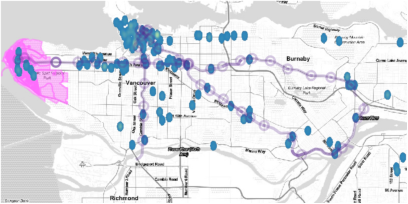
\includegraphics[width=42mm]{modo_heatmaps/min/0.pdf}
           {\\(a) 0~AM to 1~AM}
         \end{minipage}
         %\hspace{3mm}
         \begin{minipage}[b]{\linewidth}
           \centering
           \hspace*{-0.9cm}
           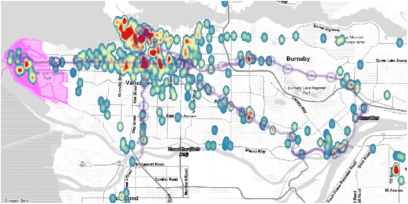
\includegraphics[width=42mm]{modo_heatmaps/min/8.pdf}
           {\\(c) 8~AM to 9~AM}
         \end{minipage}
         \begin{minipage}[b]{\linewidth}
           \centering
           \hspace*{-0.9cm}
           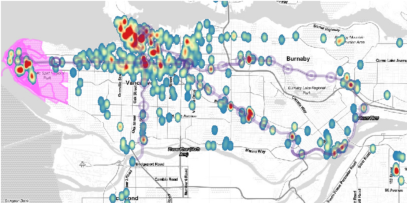
\includegraphics[width=42mm]{modo_heatmaps/min/16.pdf}
           {\\(e) 4~PM to 5~PM}
         \end{minipage}
   \end{minipage}
   \hspace{3mm}
   \begin{minipage}[b]{0.3\linewidth}
   \centering
         \begin{minipage}[b]{\linewidth}
           \centering
           \hspace*{-0.1cm}
           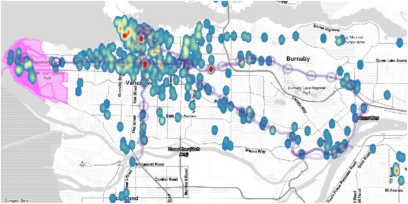
\includegraphics[width=42mm]{modo_heatmaps/min/4.pdf}
           {\\(b) 4~AM to 5~AM}
         \end{minipage}
         %\hspace{3mm}
         \begin{minipage}[b]{\linewidth}
           \centering
           \hspace*{-0.1cm}
           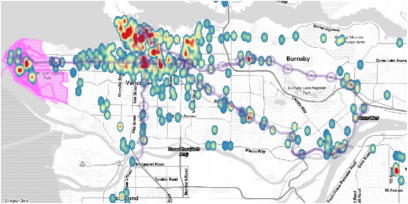
\includegraphics[width=42mm]{modo_heatmaps/min/12.pdf}
           {\\(d) 12~AM to 1~PM}
         \end{minipage}
         \begin{minipage}[b]{\linewidth}
           \hspace*{-0.1cm}
           \centering
           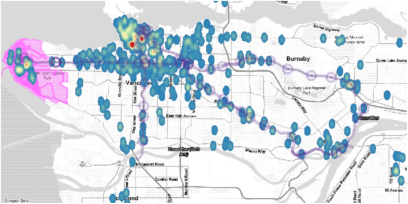
\includegraphics[width=42mm]{modo_heatmaps/min/20.pdf}
           {\\(f) 8~PM to 9~PM}
         \end{minipage}
   \end{minipage}
   \begin{minipage}[b]{0.1\linewidth}
   \centering
   		 \hspace*{12mm}
   		 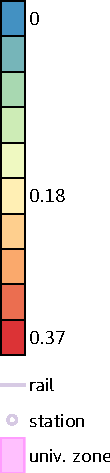
\includegraphics[width=12mm]{modo_heatmaps/legenda_modo.pdf}
         \vspace{17mm}
   \end{minipage}
   %\hspace{1cm}
   \caption{Spatial-temporal service demand for two-way service Modo.}
   \label{fig:4_4_heat_modo}
\end{figure}

%evo
% Não é o definitivo
\begin{figure}[hhh!!]
\centering
   \begin{minipage}[b]{0.3\linewidth}
   \centering      
         \begin{minipage}[b]{\linewidth}
           \hspace*{-0.9cm}
           \centering
           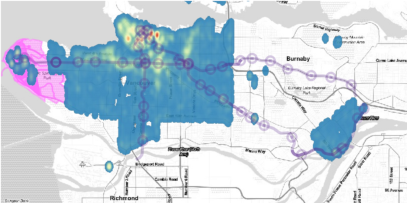
\includegraphics[width=42mm]{evo_heatmaps/min/hora0.pdf}
           {\\(a) 0~AM to 1~AM}
         \end{minipage}
         %\hspace{3mm}
         \begin{minipage}[b]{\linewidth}
           \centering
           \hspace*{-0.9cm}
           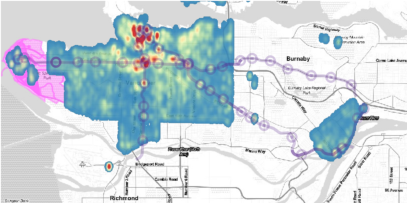
\includegraphics[width=42mm]{evo_heatmaps/min/hora8.pdf}
           {\\(c) 8~AM to 9~AM}
         \end{minipage}
         \begin{minipage}[b]{\linewidth}
           \centering
           \hspace*{-0.9cm}
           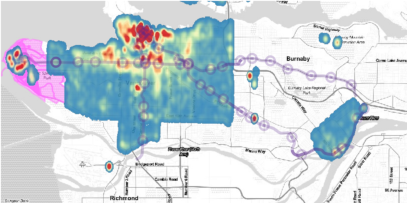
\includegraphics[width=42mm]{evo_heatmaps/min/hora16.pdf}
           {\\(e) 4~PM to 5~PM}
         \end{minipage}
   \end{minipage}
   \hspace{3mm}
   \begin{minipage}[b]{0.3\linewidth}
   \centering
         \begin{minipage}[b]{\linewidth}
           \centering
           \hspace*{-0.1cm}
           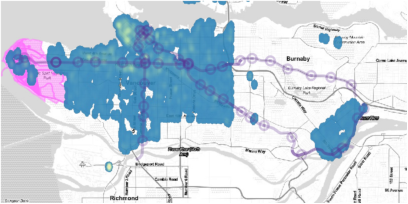
\includegraphics[width=42mm]{evo_heatmaps/min/hora4.pdf}
           {\\(b) 4~AM to 5~AM}
         \end{minipage}
         %\hspace{3mm}
         \begin{minipage}[b]{\linewidth}
           \centering
           \hspace*{-0.1cm}
           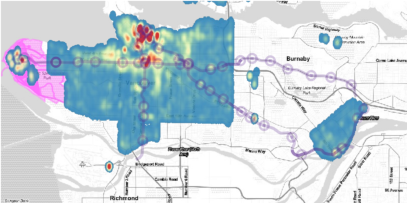
\includegraphics[width=42mm]{evo_heatmaps/min/hora12.pdf}
           {\\(d) 12~AM to 1~PM}
         \end{minipage}
         \begin{minipage}[b]{\linewidth}
           \hspace*{-0.1cm}
           \centering
           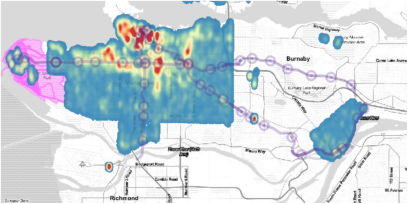
\includegraphics[width=42mm]{evo_heatmaps/min/hora20.pdf}
           {\\(f) 8~PM to 9~PM}
         \end{minipage}
   \end{minipage}
   \begin{minipage}[b]{0.1\linewidth}
   \centering
   		 \hspace*{12mm}
   		 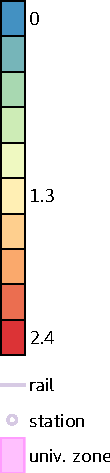
\includegraphics[width=12mm]{evo_heatmaps/legenda_evo.pdf}
         \vspace{17mm}
   \end{minipage}
   %\hspace{1cm}
   \caption{Spatial-temporal service demand for one-way service Evo.}
   \label{fig:4_4_heat_evo}
\end{figure}

% car2go
\begin{figure}[hhh!!]
\centering
   \begin{minipage}[b]{0.3\linewidth}
   \centering      
         \begin{minipage}[b]{\linewidth}
           \hspace*{-0.9cm}
           \centering
           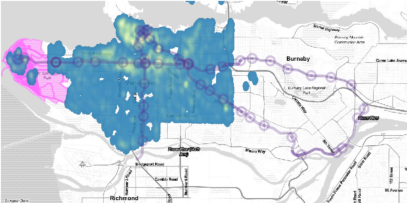
\includegraphics[width=42mm]{car2go_heatmaps/min/0.pdf}
           {\\(a) 0~AM to 1~AM}
         \end{minipage}
         %\hspace{3mm}
         \begin{minipage}[b]{\linewidth}
           \centering
           \hspace*{-0.9cm}
           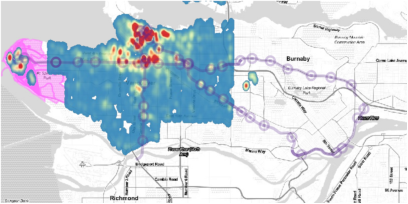
\includegraphics[width=42mm]{car2go_heatmaps/min/8.pdf}
           {\\(c) 8~AM to 9~AM}
         \end{minipage}
         \begin{minipage}[b]{\linewidth}
           \centering
           \hspace*{-0.9cm}
           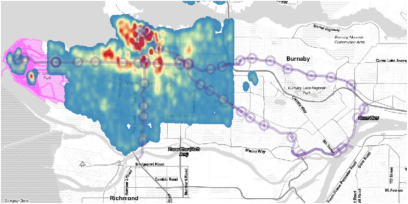
\includegraphics[width=42mm]{car2go_heatmaps/min/16.pdf}
           {\\(e) 4~PM to 5~PM}
         \end{minipage}
   \end{minipage}
   \hspace{3mm}
   \begin{minipage}[b]{0.3\linewidth}
   \centering
         \begin{minipage}[b]{\linewidth}
           \centering
           \hspace*{-0.1cm}
           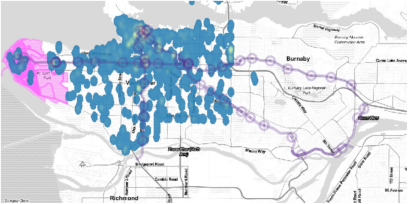
\includegraphics[width=42mm]{car2go_heatmaps/min/4.pdf}
           {\\(b) 4~AM to 5~AM}
         \end{minipage}
         %\hspace{3mm}
         \begin{minipage}[b]{\linewidth}
           \centering
           \hspace*{-0.1cm}
           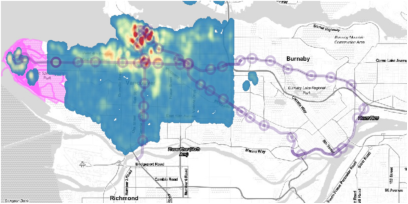
\includegraphics[width=42mm]{car2go_heatmaps/min/12.pdf}
           {\\(d) 12~AM to 1~PM}
         \end{minipage}
         \begin{minipage}[b]{\linewidth}
           \hspace*{-0.1cm}
           \centering
           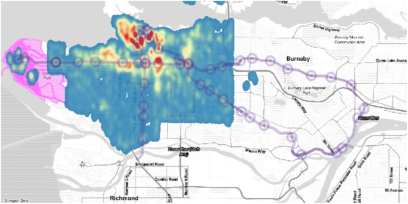
\includegraphics[width=42mm]{car2go_heatmaps/min/20.pdf}
           {\\(f) 8~PM to 9~PM}
         \end{minipage}
   \end{minipage}
   \begin{minipage}[b]{0.1\linewidth}
   \centering
   		 \hspace*{12mm}
   		 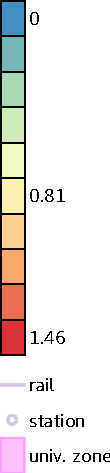
\includegraphics[width=12mm]{car2go_heatmaps/legenda_car2go.pdf}
         \vspace{17mm}
   \end{minipage}
   %\hspace{1cm}
   \caption{Spatial-temporal service demand for free-floating service Car2Go.}
   \label{fig:4_4_heat_car2go}
\end{figure}

Figures~\ref{fig:4_4_heat_modo}, \ref{fig:4_4_heat_evo} and \ref{fig:4_4_heat_car2go} present heat-maps of the hourly\footnote{Due to space constraints, we only show one-hour period every four hour.} mean number of busy vehicles in a given location, considering analyzed period. In the case of Modo, a location refers to a fixed station. In the case of the other two services, the maps present clustered travel records where users pick-up or leave a vehicle. To cluster these points the algorithm uses a 400\,m radius as a reference, forming a region close to a neighborhood. Rangin radius from 100\,m to 1000\,m, leads to similar results. 

First, all three services present a large demand in the downtown area and the university zone. Note that the demand in downtown for all three services is low during the night, starts increasing at 4-5 AM, reaches its peak during office working hours and reduces by the end of the day. In this case, users usually pick-up cars to their daily tasks, as go to work and shopping. During the night, usage increases in the surroundings of the city, the university zone, and neighborhoods with leisure facilities (such as bars). 
Modo presents a distinct demand pattern. Indeed, Modo has fixed stations located along with the existing public transport system, especially the Expo Line and Millennium Line. For this reason, it is possible to highlight a strong relationship between the existing public transport system and the car-sharing system demand. On the other hand, the other two services are more flexible. Users can rent a car almost anywhere. In this sense, despite the major demand in downtown, it is present a widespread demand all over the city.

Figures~\ref{fig:4_4_matrixEvo} and \ref{fig:4_4_matrixCar2Go} detail the spatial-temporal demand for Evo and Car2Go by presenting their origin-destination matrix mapped on 31 city areas as defined by the metropolitan city of Vancouver. To enhance the visual effects, we normalized the previous heat-maps values to a scale between 0-1, using the min-max method. Moreover, due to space constraint, this work shows the origin-destination matrix at a specific hour, i.e., at 4\,PM.
In general, the users tend to start and end a trip at the same location. It appears that during working days, users tend to use a shared car  returning it to the same region where they start (likely where they are working or living). However, for both services, a non-negligible probability to spread services along all city area is noticeable. 
Moreover, we also note that some regions serve as hubs. This is more notable for Evo service. As shown in figure~\ref{fig:4_4_matrixEvo}, the downtown area serves as a hub to start trips to almost all other regions. The opposite (a high tendency to start a trip ending at downtown) trend is not present. As a consequence, service may become unbalanced and, from time to time, service maintenance should relocate vehicles from a region to another, to accommodate the daily demand.

\begin{figure}[tbh]
\centering
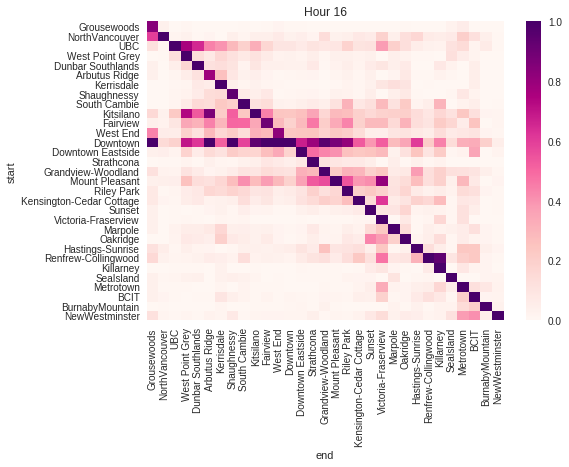
\includegraphics[width=0.85\columnwidth]{destination_matrix/hour16.png}
\caption{Origin-destination matrix for one-way service Evo (from 4~PM to 5~PM).}
\label{fig:4_4_matrixEvo}
\end{figure}
%
\begin{figure}[tbh]
\centering
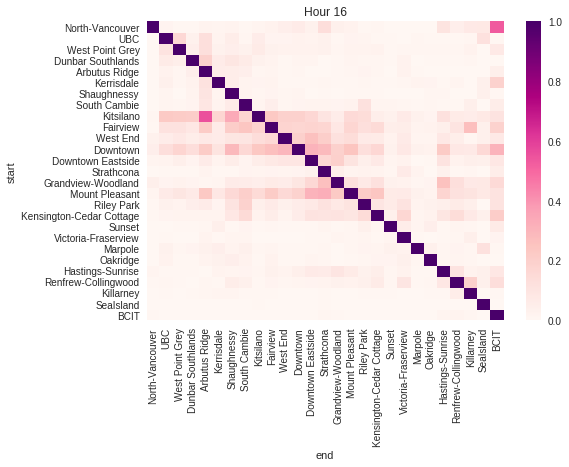
\includegraphics[width=0.85\columnwidth]{car2go_destination_matrix/hour16.png}
\caption{Origin-destination matrix for free-floating service Car2Go (from 4~PM to 5~PM).}
\label{fig:4_4_matrixCar2Go}
\end{figure}


%%%%%%%%%%%%%%%%%%%%%%%%%%%%%%%%%%%


\subsection{User behavior characteristics}
\label{sec:4_4_user-behavior}


Vehicles busy and idle periods direct impacts service revenue. Indeed, the longer the busy period is and the lower the idle period of a vehicle is, the more profitable the car will be. Therefore, the work characterizes the busy and idle periods of vehicles for all three services. In this analysis, are considered all the vehicles and all the trips lasting less than 90 minutes, which corresponds to more than 99.5\% records. 
For each service, we identified the statistical distribution that best fits the actual data (busy and idle period). For this purpose, we tested more than 40 well-known statistical distributions. More in-depth, for each component of the model, the parameters of the distribution that most closely approximate the data are determined using the Maximum Likelihood Estimation (MLE) method. After defining the parameters of each component of the model, the ten distributions with shorter Kolmogorov-Smirnov distance (continuous distributions) or lower least square error (discrete distributions) concerning the data are chosen. Finally, we chose the top three common distributions to each car-sharing service. These choices are also validated with a visual assessment of the curve fitting.

Figure~\ref{fig:4_4_busy_all_eCDF} shows the Cumulative Distribution Function of vehicle busy time.  Modo, Evo and Car2Go busy time and their best statistical distribution fitting are shown in blue, red and yellow, respectively. For all three services, the Inverse~Gamma\footnote{Cumulative distribution function (CDF) of the Inverse~Gamma distribution: $F(x, a, \beta, \delta) = \frac{1}{\Gamma(a)}\int_{1/\left((x-\beta)/\delta\right)}^{\infty}t^{a-1}e^{-t}dt$}, 
the Burr\footnote{Cumulative distribution function (CDF) of the Burr distribution: $F(x,c,d,\beta,\delta)=\left(1 + \left((x-\beta)/\delta\right)^{-c}\right)^{-d}$}, 
and Mielke's Beta-Kappa\footnote{Cumulative distribution function (CDF) of the Mielke's Beta-Kappa distribution: $F(x,k,s,\beta,\delta) = \frac{\left((x-\beta)/\delta\right)^{k}}{(1+\left((x-\beta)/\delta\right)^{s})^{(k*\frac{1}{s})}}$} 
distributions present a  good fitting to the empirical data, with similar MLEs.  
Table~\ref{table:fit_busy} summarizes the parameters of the distributions of the busy time for each statistical distribution.
Despite all three services present the same statistical distribution fitting, 
the two-way service (i.e., Modo), presents a clear shift to right on its curve when compared to the other two services, as shown in Figure~\ref{fig:4_4_busy_all_eCDF}. As we previously discussed, the median busy time on Modo is more than one hour longer than the median busy time for the other services. 
Users in Modo must return cars to the same station they originated travels. As a consequence, they tend to perform longer tasks. On the other hand, with the other two services users tend to do a longer number of shorter travels.

Finally, figure~\ref{fig:4_4_idle_all_eCDF}, presents vehicle idle periods distribution.  Power~log~normal\footnote{Cumulative distribution function (CDF) of the Power~log~normal distribution: $F(x,c,s,\beta,\delta)=1-\left(\frac{1}{\sqrt{2\pi}}\int_{-\infty}^{-log((x-\beta)/\delta)/s}e^{-t^{2}/2}dt\right)^{c}$}, Burr and Mielke's~Beta$-$Kappa distributions best fit the idle data, for all three datasets. Table~\ref{table:fit_idle} presents the distribution parameters. 
Again, Modo presents a distinct behavior from the other two services. The longer idle period for Modo vehicles corroborates to our previous observations. Indeed, the demand for car-sharing varies over the city during a day. While users in Evo and Car2Go can park anywhere, they contribute to spreading cars over the city. For example, at least 75\% of cars in Modo remains idle for periods longer than 2 hours. For the other two services, no more than 20\% of vehicles remains idle for the same period.

In sum, our analysis shows that the free-floating and one-way car-sharing systems have similar characteristics. They are mostly used for short/medium period travels, while the two-way system is mostly used for medium to long travels. 
Moreover, Evo and Car2Go dynamically spread car over the city, turning the car's idle periods shorter. The longer number of shorter travels, associated with the shorter idle periods, may indicate a more profitable service.

\begin{figure}[tbh]
   \centering
   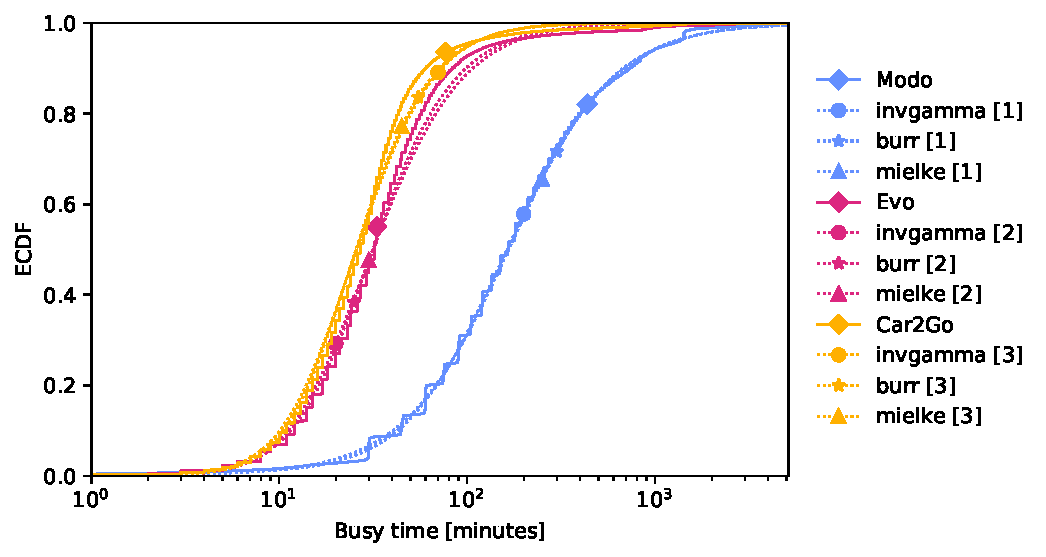
\includegraphics[width=0.85\columnwidth]{images_test/CDF_Fit_final.pdf}
   \caption{Cumulative distribution function of vehicle busy time.}
   \label{fig:4_4_busy_all_eCDF}
\end{figure}


\begin{table}
\centering
\setlength{\tabcolsep}{2.3pt}
	\begin{tabular}{lll}
	\hline
	\multirow{3}{*}{Modo}   & Inv.Gamma       & a = 1.7032,  $\beta$ = -38.5120,  $\delta$ = 278.8487                        \\
	                        & Burr                & c = 1.5651, d = 1.0327,  $\beta$ = -1.8893, $\delta$ = 163.0525 \\
	                        & Mielke & k = 1.59745, s = 1.5687,  $\beta$ = -1.6713, $\delta$ = 164.9877 \\ \hline
	\multirow{3}{*}{Evo}    & Inv.Gamma       & a = 2.0674, $\beta$ = -4.7928, $\delta$ = 63.4382                          \\
	                        & Burr                & c = 1.8332, d = 1.5078, $\beta$ = -0.1855, $\delta$ = 23.5794   \\
	                        & Mielke & k = 2.7305, s = 1.8336, $\beta$ = -0.1125, $\delta$ = 23.7291 \\ \hline
	\multirow{3}{*}{Car2Go} & Inv.Gamma       & a = 2.7688, $\beta$ = -4.9702, $\delta$ = 75.2494                           \\
	                        & Burr                & c = 2.3869, d = 64.2072, $\beta$ = -12.5240, $\delta$ = 5.7419   \\
	                        & Mielke & k = 37.8163, s = 2.3450, $\beta$ = -10.9187, $\delta$ = 9.6407   \\ \hline
	\end{tabular}
\caption{Distributions parameters of the busy time fit curves. The $\beta$ and $\delta$ are key parameters to adjust the location and scale of the distributions.}
\label{table:fit_busy}
\end{table}

\begin{figure}
   \centering
   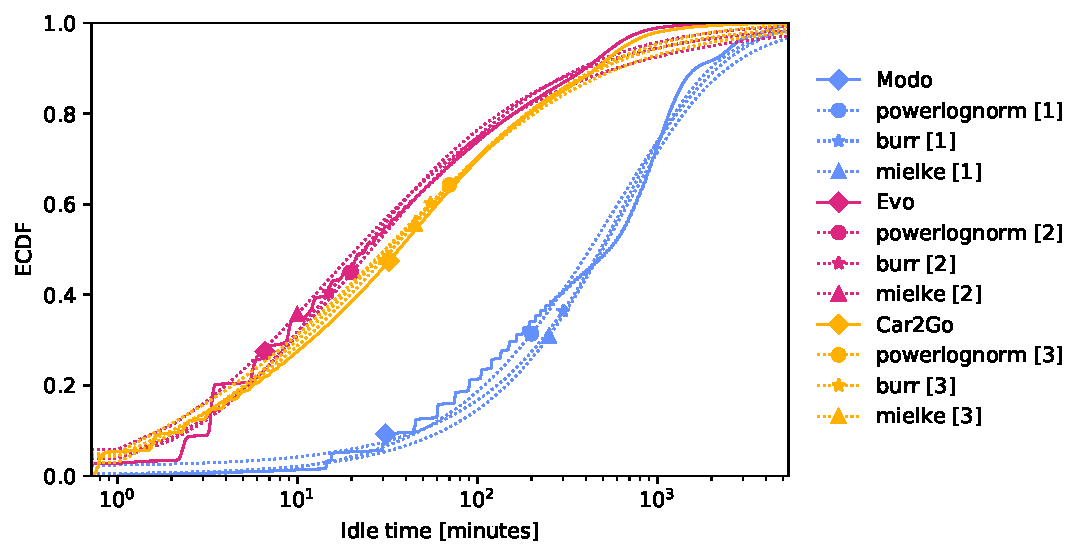
\includegraphics[width=0.85\columnwidth]{images_test/CDF_Fit_idle_final.pdf}
   \caption{Cumulative distribution function of vehicle idle time}
   \label{fig:4_4_idle_all_eCDF}
\end{figure}


\begin{table}
\centering
\setlength{\tabcolsep}{2.3pt}
	\begin{tabular}{lll}
	\hline
	\multirow{3}{*}{Modo}   & PLogNorm       & c = 118.7142, s=3.6088,  $\beta$=0.7191,  $\delta$=3780209.5149                     \\
	                        & Burr                & c = 1.9865, d = 0.3860,  $\beta$ = -7.7229, $\delta$ = 1105.5853 \\
	                        & Mielke & k = 0.8898, s = 1.5390,  $\beta$ = -1.4862, $\delta$ = 860.6790 \\ \hline
	\multirow{3}{*}{Evo}    & PLogNorm       & c = 0.0723, s = 0.7003,  $\beta$ = -0.6723,  $\delta$ = 1.8246                          \\
	                        & Burr                & c = 0.6931, d = 3.7574, $\beta$ = -0.4881, $\delta$ = 2.3713   \\
	                        & Mielke & k = 2.7161, s = 0.5882, $\beta$ = -0.2800, $\delta$ = 0.9725 \\ \hline
	\multirow{3}{*}{Car2Go} & PLogNorm       & c = 4.8747, s = 3.3741,  $\beta$ = 0.7134,  $\delta$ = 1334.7243                           \\
	                        & Burr                & c = 0.7714, d = 0.7337, $\beta$ = 0.7166, $\delta$ = 53.9727   \\
	                        & Mielke & k = 0.5743, s = 0.8826, $\beta$ = 0.7166, $\delta$ = 68.1029   \\ \hline
	\end{tabular}
\caption{Distributions parameters of the idle time fit curves. The $\beta$ and $\delta$ are keyword parameters to adjust the location and scale of the distributions.}	\label{table:fit_idle}

\end{table}

